\documentclass[bachelor, och, labwork]{shiza}
% параметр - тип обучения - одно из значений:
%    spec     - специальность
%    bachelor - бакалавриат (по умолчанию)
%    master   - магистратура
% параметр - форма обучения - одно из значений:
%    och   - очное (по умолчанию)
%    zaoch - заочное
% параметр - тип работы - одно из значений:
%    referat    - реферат
%    coursework - курсовая работа (по умолчанию)
%    diploma    - дипломная работа
%    pract      - отчет по практике
% параметр - включение шрифта
%    times    - включение шрифта Times New Roman (если установлен)
%               по умолчанию выключен
\usepackage{subfigure}
\usepackage{tikz,pgfplots}
\pgfplotsset{compat=1.5}
\usepackage{float}

%\usepackage{titlesec}
\setcounter{secnumdepth}{4}
%\titleformat{\paragraph}
%{\normalfont\normalsize}{\theparagraph}{1em}{}
%\titlespacing*{\paragraph}
%{35.5pt}{3.25ex plus 1ex minus .2ex}{1.5ex plus .2ex}

\titleformat{\paragraph}[block]
{\hspace{1.25cm}\normalfont}
{\theparagraph}{1ex}{}
\titlespacing{\paragraph}
{0cm}{2ex plus 1ex minus .2ex}{.4ex plus.2ex}

% --------------------------------------------------------------------------%


\usepackage[T2A]{fontenc}
\usepackage[utf8]{inputenc}
\usepackage{graphicx}
\graphicspath{ {./images/} }
\usepackage{tempora}

\usepackage[sort,compress]{cite}
\usepackage{amsmath}
\usepackage{amssymb}
\usepackage{amsthm}
\usepackage{fancyvrb}
\usepackage{listings}
\usepackage{listingsutf8}
\usepackage{longtable}
\usepackage{array}
\usepackage[english,russian]{babel}

\usepackage[colorlinks=false]{hyperref}
\usepackage{url}

\usepackage{underscore}
\usepackage{setspace}
\usepackage{indentfirst} 
\usepackage{mathtools}
\usepackage{amsfonts}
\usepackage{enumitem}
\usepackage{tikz}
\usepackage{minted}


\newcommand{\eqdef}{\stackrel {\rm def}{=}}
\newcommand{\specialcell}[2][c]{%
\begin{tabular}[#1]{@{}c@{}}#2\end{tabular}}

\renewcommand\theFancyVerbLine{\small\arabic{FancyVerbLine}}

\newtheorem{lem}{Лемма}

\begin{document}

% Кафедра (в родительном падеже)
\chair{теоретических основ компьютерной безопасности и криптографии}

% Тема работы
\title{Решение систем линейных уравнений методом Гаусса}

% Курс
\course{3}

% Группа
\group{331}

% Факультет (в родительном падеже) (по умолчанию "факультета КНиИТ")
\department{факультета КНиИТ}

% Специальность/направление код - наименование
%\napravlenie{09.03.04 "--- Программная инженерия}
%\napravlenie{010500 "--- Математическое обеспечение и администрирование информационных систем}
%\napravlenie{230100 "--- Информатика и вычислительная техника}
%\napravlenie{231000 "--- Программная инженерия}
\napravlenie{10.05.01 "--- Компьютерная безопасность}

% Для студентки. Для работы студента следующая команда не нужна.
% \studenttitle{Студентки}

% Фамилия, имя, отчество в родительном падеже
\author{Токарева Никиты Сергеевича}

% Заведующий кафедрой
% \chtitle{} % степень, звание
% \chname{}

%Научный руководитель (для реферата преподаватель проверяющий работу)
\satitle{доцент} %должность, степень, звание
\saname{А. Н. Гамова}

% Руководитель практики от организации (только для практики,
% для остальных типов работ не используется)
% \patitle{к.ф.-м.н.}
% \paname{С.~В.~Миронов}

% Семестр (только для практики, для остальных
% типов работ не используется)
%\term{8}

% Наименование практики (только для практики, для остальных
% типов работ не используется)
%\practtype{преддипломная}

% Продолжительность практики (количество недель) (только для практики,
% для остальных типов работ не используется)
%\duration{4}

% Даты начала и окончания практики (только для практики, для остальных
% типов работ не используется)
%\practStart{30.04.2019}
%\practFinish{27.05.2019}

% Год выполнения отчета
\date{2022}

\maketitle

% Включение нумерации рисунков, формул и таблиц по разделам
% (по умолчанию - нумерация сквозная)
% (допускается оба вида нумерации)
% \secNumbering

%-------------------------------------------------------------------------------------------

\tableofcontents


\section{Описание алгоритма}

  Метод Гаусса — классический метод решения системы линейных алгебраических уравнений (СЛАУ).Рассмотрим систему линейных уравнений с действительными постоянными коэффициентами:

  \begin{equation*}
    \begin{cases}
      a_{11} \cdot x_1 +  a_{12} \cdot x_2 + \ldots + a_{1n} \cdot x_n = y_1 \\
      a_{21} \cdot x_1 + a_{22} \cdot x_2 + \ldots + a_{2n} \cdot x_n = y_2 \\
      \ldots \\
      a_{n1} \cdot x_1 + a_{n2} \cdot x_2 + \ldots + a_{nn} \cdot x_n = y_n
    \end{cases}
  \end{equation*}

  Метод Гаусса решения системы линейных уравнений включает в себя 2 стадии:

  \begin{itemize}
    \item последовательное (прямое) исключение;
    \item обратная подстановка.
  \end{itemize}

  \subsection{Последовательное исключение}
    Последовательное исключение
    Исключения Гаусса основаны на идее последовательного исключения переменных по одной до тех пор, пока не
    останется только одно уравнение с одной переменной в левой части. Затем это уравнение решается относительно
    единственной переменной. Таким образом, систему уравнений приводят к треугольной (ступенчатой) форме. Для
    этого среди элементов первого столбца матрицы выбирают ненулевой (а чаще максимальный) элемент и перемещают
    его на крайнее верхнее положение перестановкой строк. Затем нормируют все уравнения, разделив его на
    коэффициент $a_{i1}$, где $i$ -- номер строки.
  
    \begin{equation*}
      \begin{cases}
        x_1 +  \frac{a_{12}}{a_{11}} \cdot x_2 + \ldots + \frac{a_{1n}}{a_{11}} \cdot x_n = \frac{y_1}{a_{11}} \\
        x_1 +  \frac{a_{22}}{a_{21}} \cdot x_2 + \ldots + \frac{a_{2n}}{a_{21}} \cdot x_n = \frac{y_2}{a_{21}} \\
        \ldots \\
        x_1 +  \frac{a_{n2}}{a_{n1}} \cdot x_2 + \ldots + \frac{a_{nn}}{a_{n1}} \cdot x_n = \frac{y_n}{a_{n1}} \\
      \end{cases}
    \end{equation*}

    Затем вычитают получившуюся после перестановки первую строку из остальных строк:

    \begin{equation*}
      \begin{cases}
        x_1 +  \frac{a_{12}}{a_{11}} \cdot x_2  + \ldots + \frac{a_{1n}}{a_{11}} \cdot x_n = \frac{y_1}{a_{11}} \\
        0 +  (\frac{a_{22}}{a_{21}} - \frac{a_{12}}{a_{11}}) \cdot x_2 + \ldots + (\frac{a_{2n}}{a_{21}} - \frac{a_{1n}}{a_{11}}) \cdot x_n = (\frac{y_2}{a_{21}} - \frac{y_1}{a_{11}}) \\
        \ldots \\
        0 +  (\frac{a_{n2}}{a_{n1}} - \frac{a_{12}}{a_{11}}) \cdot x_2 + \ldots + (\frac{a_{nn}}{a_{n1}} - \frac{a_{1n}}{a_{11}}) \cdot x_n = (\frac{y_n}{a_{n1}} - \frac{y_1}{a_{11}}) \\
      \end{cases}
    \end{equation*}

    Получают новую систему уравнений, в которой заменены соответствующие коэффициенты.

    \begin{equation*}
      \begin{cases}
        x_1 +  a_{12}^{'} \cdot x_2 + \ldots + a_{1n}^{'} \cdot x_n = y_1^{'} \\
        0 +  a_{22}^{'} \cdot x_2 + \ldots + a_{2n}^{'} \cdot x_n = y_2^{'} \\
        \ldots \\
        0 +  a_{n2}^{'} \cdot x_2 + \ldots + a_{nn}^{'} \cdot x_n = y_n^{'} \\
      \end{cases}
    \end{equation*}

    После того, как указанные преобразования были совершены, первую строку и первый столбец мысленно
    вычёркивают и продолжают указанный процесс для всех последующих уравнений пока не останется уравнение с одной неизвестной:

    \begin{equation*}
      \begin{cases}
        x_1 + a_{12}^{'} \cdot x_2 + a_{13}^{'} \cdot x_3 + \ldots + a_{1n}^{'} \cdot x_n = y_1^{'} \\
        0 + x_2 + a_{23}^{''} \cdot x_3 + \ldots + a_{2n}^{''} \cdot x_n = y_2^{''} \\
        0 + 0 + x_3 + \ldots + a_{2n}^{'''} \cdot x_n = y_3^{'''} \\
        \ldots \\
        0 + 0 + 0 + \ldots + x_n = y_n^{n_{'}} \\
      \end{cases}
    \end{equation*}
  
  \subsection{Обратная подстановка}
  
  Обратная подстановка предполагает подстановку полученного на предыдущем шаге значения переменной $x_n$ в предыдущие уравнения:

  \begin{center}
    $x_{n-1} = y_{n-1}^{(n-1)'} - a_{(n-1)n}^{(n-1)'} \cdot x_n$
    
    $x_{n-2} + a_{(n-2)(n-1)}^{(n-2)'} \cdot x_{n-1} = y_{n-2}^{(n-2)'} - a_{(n-2)n}^{(n-2)'} \cdot x_n$

    $\ldots$

    $x_2 + a_{23}^{''} \cdot x_3 + \ldots + a_{2(n-1)}^{''} \cdot x_{n-1} = y_2^{''} - a_{2n}^{''} \cdot x_n$

    $x_1 + a_{12}^{'} \cdot x_2 + a_{13}^{'} \cdot x_3 + \ldots + a_{1(n-1)}^{'} \cdot x_{n-1} = y_1^{'} - a_{1n}^{'} \cdot x_n$
    
  \end{center}

  Эта процедура повторяется для всех оставшихся решений:

  \begin{center}    
    $x_{n-2} = (y_{n-2}^{(n-2)'} - a_{(n-2)n}^{(n-2)'} \cdot x_n) - a_{(n-2)(n-1)}^{(n-2)'} \cdot x_{n-1}$

    $\ldots$

    $x_2 + a_{23}^{''} \cdot x_3 + \ldots = (y_2^{''} - a_{2n}^{''} \cdot x_n) - a_{2(n-1)}^{''} \cdot x_{n-1}$

    $x_1 + a_{12}^{'} \cdot x_2 + a_{13}^{'} \cdot x_3 + \ldots = (y_1^{'} - a_{1n}^{'} \cdot x_n) - a_{1(n-1)}^{'} \cdot x_{n-1}$
    
  \end{center}

\section{Код программы, реализующий алгоритм}

  Далее представлена реализация алгоритма решения системы линейных уравнений методом Гаусса, написанная на языке $C++$.

  \inputminted[fontsize=\small]{C++}{code/gauss.cpp}

  Далее приведем пример, подав в качестве входных данных коэффициенты системы линейных уравнений (СЛУ), чтобы проверить корректность, написанного
  кода.

  Решим следующую СЛУ:
  
  \begin{equation*}
    \begin{cases}
      3 \cdot x_1 + 2 \cdot x_2 - 5 \cdot x_3 = -1 \\
      2 \cdot x_1 - 1 \cdot x_2 + 3 \cdot x_3 = 13 \\
      1 \cdot x_1 + 2 \cdot x_2 - 1 \cdot x_3 = 9 \\
    \end{cases}
  \end{equation*}
  
  На рисунке 1 показан ввод значений коэффициентов, и вывод решения СЛУ.
  
  \begin{figure}[H]
    \centering
    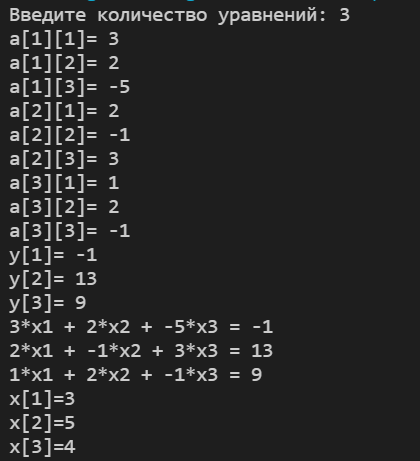
\includegraphics[width=0.8\textwidth]{img/3-1}
    \caption{Результат работы алгоритма}
  \end{figure}

  Проверим полученные выходные данные, подставив эти значения в СЛУ. Как видно из данной подстановки,
  значения $x_1, x_2, x_3$ были найдены корректно. 

  \begin{equation*}
    \begin{cases}
      3 \cdot 3 + 2 \cdot 5 - 5 \cdot 4 = -1 \\
      2 \cdot 3 - 1 \cdot 5 + 3 \cdot 4 = 13 \\
      1 \cdot 3 + 2 \cdot 5 - 1 \cdot 4 = 9 \\
    \end{cases}
  \end{equation*}
  
\section{Анализ алгоритма}

  Для того, чтобы алгоритм работал корректно, необходимо пройти по всем $n$ уравнениям ($O(n)$). С учетом оценки 
  сложности поиска максимального элемента и перестановки строки, содержащей этот опорный элемент, равной $O(n+n)= O(n)$.
  и оценки сложности нормализации уравнений, равной $O(n^2)$,  итоговая оценка сложности равна $O(n \cdot (n^2 + n)) = O(n^3)$.
  
\conclusion

В данной лабораторной работе был рассмотрен алгоритм решения систем линейных уравнений методом Гаусса и был проведен анализ оценки его сложности.
Это послужило созданием её программной реализации, написанной на языке $C++$. 

\begin{thebibliography}{3}
  \bibitem{1}
  Статья "Решение систем линейных уравнений методом Гаусса"  / [Электронный ресурс] URL: https://function-x.ru/systems_gauss.html (дата обращения 27.02.2022), Яз. рус
  \bibitem{2}
  Книга Маховенко Е.Б. "Теоретико-числовые методы в криптографии", Москва, "Гелиос АРВ", 2006 г., Яз. рус.
\end{thebibliography}

\end{document}
